\chapter{Introduction}

\fxnote{write intro section.}
Hi, my name is Stereo Mike.

Yeah, we got three tickets to the Bran Van concert this Monday night at the Pacific Pallisades. You can all dial in if you want to answer a couple of questions; namely, what is Todd's favorite cheese? Jackie just called up and said it was a form of Roquefort. We'll see about that.

Give us a ring ding ding, it's a beautiful day.

Yeah Todd, this is Liquid, ring-a-ding-a-dinging, I want those three Bran Van tickets, man. Whaddya think? Todd?

\section{Algorithmic Trading}

\fxnote{write algo trading section.}

\section{Limit Order Book Dynamics}


\fxnote{write LOB dynamics section }

Limit order book imbalance is a ratio of limit order volumes between the bid and ask side, and can be calculated for example as $I(t) = \dfrac{V_b(t) - V_a(t)}{V_b(t) + V_a(t)} \in [-1,1]$.
\begin{itemize}
\item We bin the bid/ask volume imbalances in the Limit Order Book into $K$ bins, each being dubbed a ``regime'' of the limit order book. 
\item $Z_t$ is a continuous-time Markov chain that tracks which regime we're in. $Z_t$ takes values in $\{1, \dots , K\}$, and has an infinitesimal generator matrix $G$.
\item Conditional on being in some regime $k$, the arrival of buy and sell market orders follow independent Poisson processes with intensities $\lambda^{\pm}_k$.
\end{itemize}

We have observations of arrivals of buy/sell market orders and of regime switches occurring, all of which are timestamped. Pictorially, a timeline might look like:
\begin{figure}[H]
  \tikzsetnextfilename{LOBtimeline}
  % Limit Order Book timeline by Anton
%

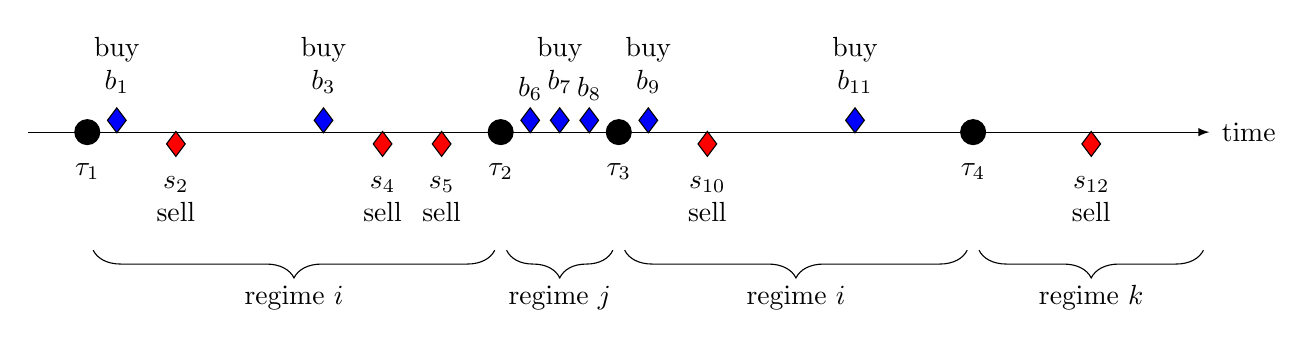
\begin{tikzpicture}[scale=1.5]
	[triangle/.style = {fill=blue!20, regular polygon, regular polygon sides=3 },
	border rotated/.style = {shape border rotate=180}]
	
    \draw [>=latex,->] (0,0) -- (10,0) node[draw=none,fill=none,shift=(right:0.5)] {time};
    \draw[mark options={fill=black}, mark size=+3pt] plot[mark=*] coordinates {(.5,0)} node[shift=(down:0.5), align=center] {$\tau_1$};
    \draw[mark options={fill=black}, mark size=+3pt] plot[mark=*] coordinates {(4,0)} node[shift=(down:0.5), align=center] {$\tau_2$};
    \draw[mark options={fill=black}, mark size=+3pt] plot[mark=*] coordinates {(5,0)} node[shift=(down:0.5), align=center] {$\tau_3$};
    \draw[mark options={fill=black}, mark size=+3pt] plot[mark=*] coordinates {(8,0)} node[shift=(down:0.5), align=center] {$\tau_4$};
    
    
	\draw[mark options={fill=blue}, mark size =+3pt, shift=(up:0.1)] plot[mark=diamond*] coordinates {(.75,0)} node[shift=(up:0.7), align=center] {buy \\ $b_1$};
	\draw[mark options={fill=red}, mark size =+3pt, shift=(down:0.1)] plot[mark=diamond*] coordinates {(1.25,0)} node[shift=(down:0.7), align=center] {$s_2$ \\ sell};
	\draw[mark options={fill=blue}, mark size =+3pt, shift=(up:0.1)] plot[mark=diamond*] coordinates {(2.5,0)} node[shift=(up:0.7), align=center] {buy \\ $b_3$};
	\draw[mark options={fill=red}, mark size =+3pt, shift=(down:0.1)] plot[mark=diamond*] coordinates {(3,0)} node[shift=(down:0.7), align=center] {$s_4$ \\ sell};
	\draw[mark options={fill=red}, mark size =+3pt, shift=(down:0.1)] plot[mark=diamond*] coordinates {(3.5,0)} node[shift=(down:0.7), align=center] {$s_5$ \\ sell};

%%% REGIME SWITCH
	
	\draw[mark options={fill=blue}, mark size =+3pt, shift=(up:0.1)] plot[mark=diamond*] coordinates {(4.25,0)} node[shift=(up:0.4), align=center] {$b_6$};
	\draw[mark options={fill=blue}, mark size =+3pt, shift=(up:0.1)] plot[mark=diamond*] coordinates {(4.50,0)} node[shift=(up:0.7), align=center]
{buy \\ $b_7$};
	\draw[mark options={fill=blue}, mark size =+3pt, shift=(up:0.1)] plot[mark=diamond*] coordinates {(4.75,0)} node[shift=(up:0.4), align=center] {$b_8$};
	
%%% REGIME SWITCH

	\draw[mark options={fill=blue}, mark size =+3pt, shift=(up:0.1)] plot[mark=diamond*] coordinates {(5.25,0)} node[shift=(up:0.7), align=center] {buy \\ $b_9$};
	\draw[mark options={fill=red}, mark size =+3pt, shift=(down:0.1)] plot[mark=diamond*] coordinates {(5.75,0)} node[shift=(down:0.7), align=center] {$s_{10}$ \\ sell};
	\draw[mark options={fill=blue}, mark size =+3pt, shift=(up:0.1)] plot[mark=diamond*] coordinates {(7,0)} node[shift=(up:0.7), align=center] {buy \\ $b_{11}$};
	
%%% REGIME SWITCH

	\draw[mark options={fill=red}, mark size =+3pt, shift=(down:0.1)] plot[mark=diamond*] coordinates {(9,0)} node[shift=(down:0.7), align=center] {$s_{12}$ \\ sell};
	
%%% BRACES
	
	\draw [decorate, decoration = {brace, amplitude = 10pt, mirror}]
	(0.55,-1) -- (3.95,-1) node [black, midway, yshift = -0.6cm] {regime $i$};
	\draw [decorate, decoration = {brace, amplitude = 10pt, mirror}]
	(4.05,-1) -- (4.95,-1) node [black, midway, yshift = -0.6cm] {regime $j$}; 
	\draw [decorate, decoration = {brace, amplitude = 10pt, mirror}]
	(5.05,-1) -- (7.95,-1) node [black, midway, yshift = -0.6cm] {regime $i$}; 
	\draw [decorate, decoration = {brace, amplitude = 10pt, mirror}]
	(8.05,-1) -- (9.95,-1) node [black, midway, yshift = -0.6cm] {regime $k$}; 
\end{tikzpicture}

\caption{Hypothetical timeline of market orders arriving during changing order imbalance regimes.}
\label{introtimeline}
\end{figure}

\section{ITCH Data Set}
\fxnote{write ITCH data set section.}